\documentclass[a4paper]{article}
\usepackage[utf8]{inputenc}
\usepackage[english]{babel}
\usepackage{moreverb}
\usepackage{graphicx}
\title{Project Report \\ EDA216 Database Technology \\ Krusty Kookies AB}
\date{\today}
\author{Fredrik Paulsson \\ dat11fp1@student.lu.se \and Jonas Jacobsson \\ dat11jja@student.lu.se}
%\setcounter{secnumdepth}{5}
%\setcounter{tocdepth}{5}
\begin{document}
\maketitle
%\tableofcontents

\section{E/R Model}
\begin{figure}[!h]
\centering
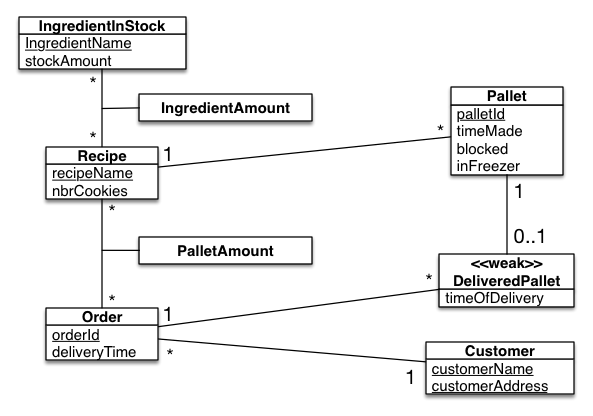
\includegraphics[scale=0.7]{projectUMLFinal.png}
\caption{UML diagram for the E/R model.}
\label{uml}
\end{figure}

\section{Relations}
\begin{description}
\item{\texttt{IngredientsInStock(\underline{ingredientName},stockAmount)}}
\item{\texttt{Recipes(\underline{recipeName},nbrCookies)}}
\item{\texttt{IngredientsInRecipe(\underline{\textit{ingredientName},\textit{recipeName}},ingredientAmount)}}
\item{\texttt{Customers(\underline{customerName,customerAddress})}}
\item{\texttt{Orders(\underline{orderId},deliveryTime,\textit{customerName,customerAddress})}}
\item{\texttt{RecipesInOrders(\underline{\textit{recipeName},\textit{orderId}},palletAmount)}}
\item{\texttt{Pallets(\underline{palletId},timeMade,blocked,inFreezer,\textit{recipeName})}}
\item{\texttt{DeliveredPallets(\underline{\textit{palletId}},timeOfDelivery,\textit{orderId})}}
\end{description}
%\begin{thebibliography}{1}
%\bibitem{wikipedia}
%http://en.wikipedia.org
%\end{thebibliography}
\end{document}